\documentclass[11pt]{article}

\usepackage[margin=1in]{geometry}
\usepackage{amsmath,amssymb,amsthm}
\usepackage{booktabs}
\usepackage{array}
\usepackage{makecell}
\usepackage{graphicx}
\renewcommand\theadalign{bc}
\renewcommand\theadfont{\bfseries\small}
\renewcommand\theadgape{\Gape[2pt]}
\renewcommand\cellgape{\Gape[2pt]}
\usepackage{microtype}
\usepackage{hyperref}
\hypersetup{colorlinks=true, linkcolor=black, urlcolor=blue, citecolor=black}
\usepackage[capitalize,noabbrev]{cleveref}
\usepackage{enumitem}
\setlist{nosep,leftmargin=*}
\usepackage{caption}
\captionsetup{font=small, labelfont=bf, skip=4pt}

\newcommand{\E}{\mathbb{E}}
\newcommand{\Prob}{\mathbb{P}}
\newcommand{\indicator}[1]{\mathbf{1}\{#1\}}
\newcommand{\fhat}{\widehat{f}}
\newcommand{\ghat}{\widehat{g}}
\newcommand{\that}{\widehat{t}}
\newcommand{\Vhat}{\widehat{V}}
\newcommand{\CVaR}{\mathrm{CVaR}}
\renewcommand{\thefootnote}{\fnsymbol{footnote}}

\title{CVaR-CJE Pilot on HealthBench}
\author{}
\date{}

\begin{document}
\maketitle
\thispagestyle{empty}
\vspace{-2.5em}

\paragraph{TL;DR.}
A cheap LLM judge plus a small oracle slice can estimate worst-tail policy
quality, and a two-moment transport audit decides when to trust the number.
Across five HealthBench policies graded by gpt-4o-mini against gpt-4.1, the
calibrated Direct $\CVaR$-CJE estimate is closer to the full-oracle truth than
the cheap-only baseline on every cell, mean $|err|$ drops from $0.126$
(cheap-only) to $0.047$ (Direct) at $\alpha = 0.10$, and the audit refuses
the worst miss the estimator would otherwise make. \Cref{fig:mvp} summarizes
the picture in one chart; the rest of the paper unpacks it.

\begin{figure}[h]
\centering
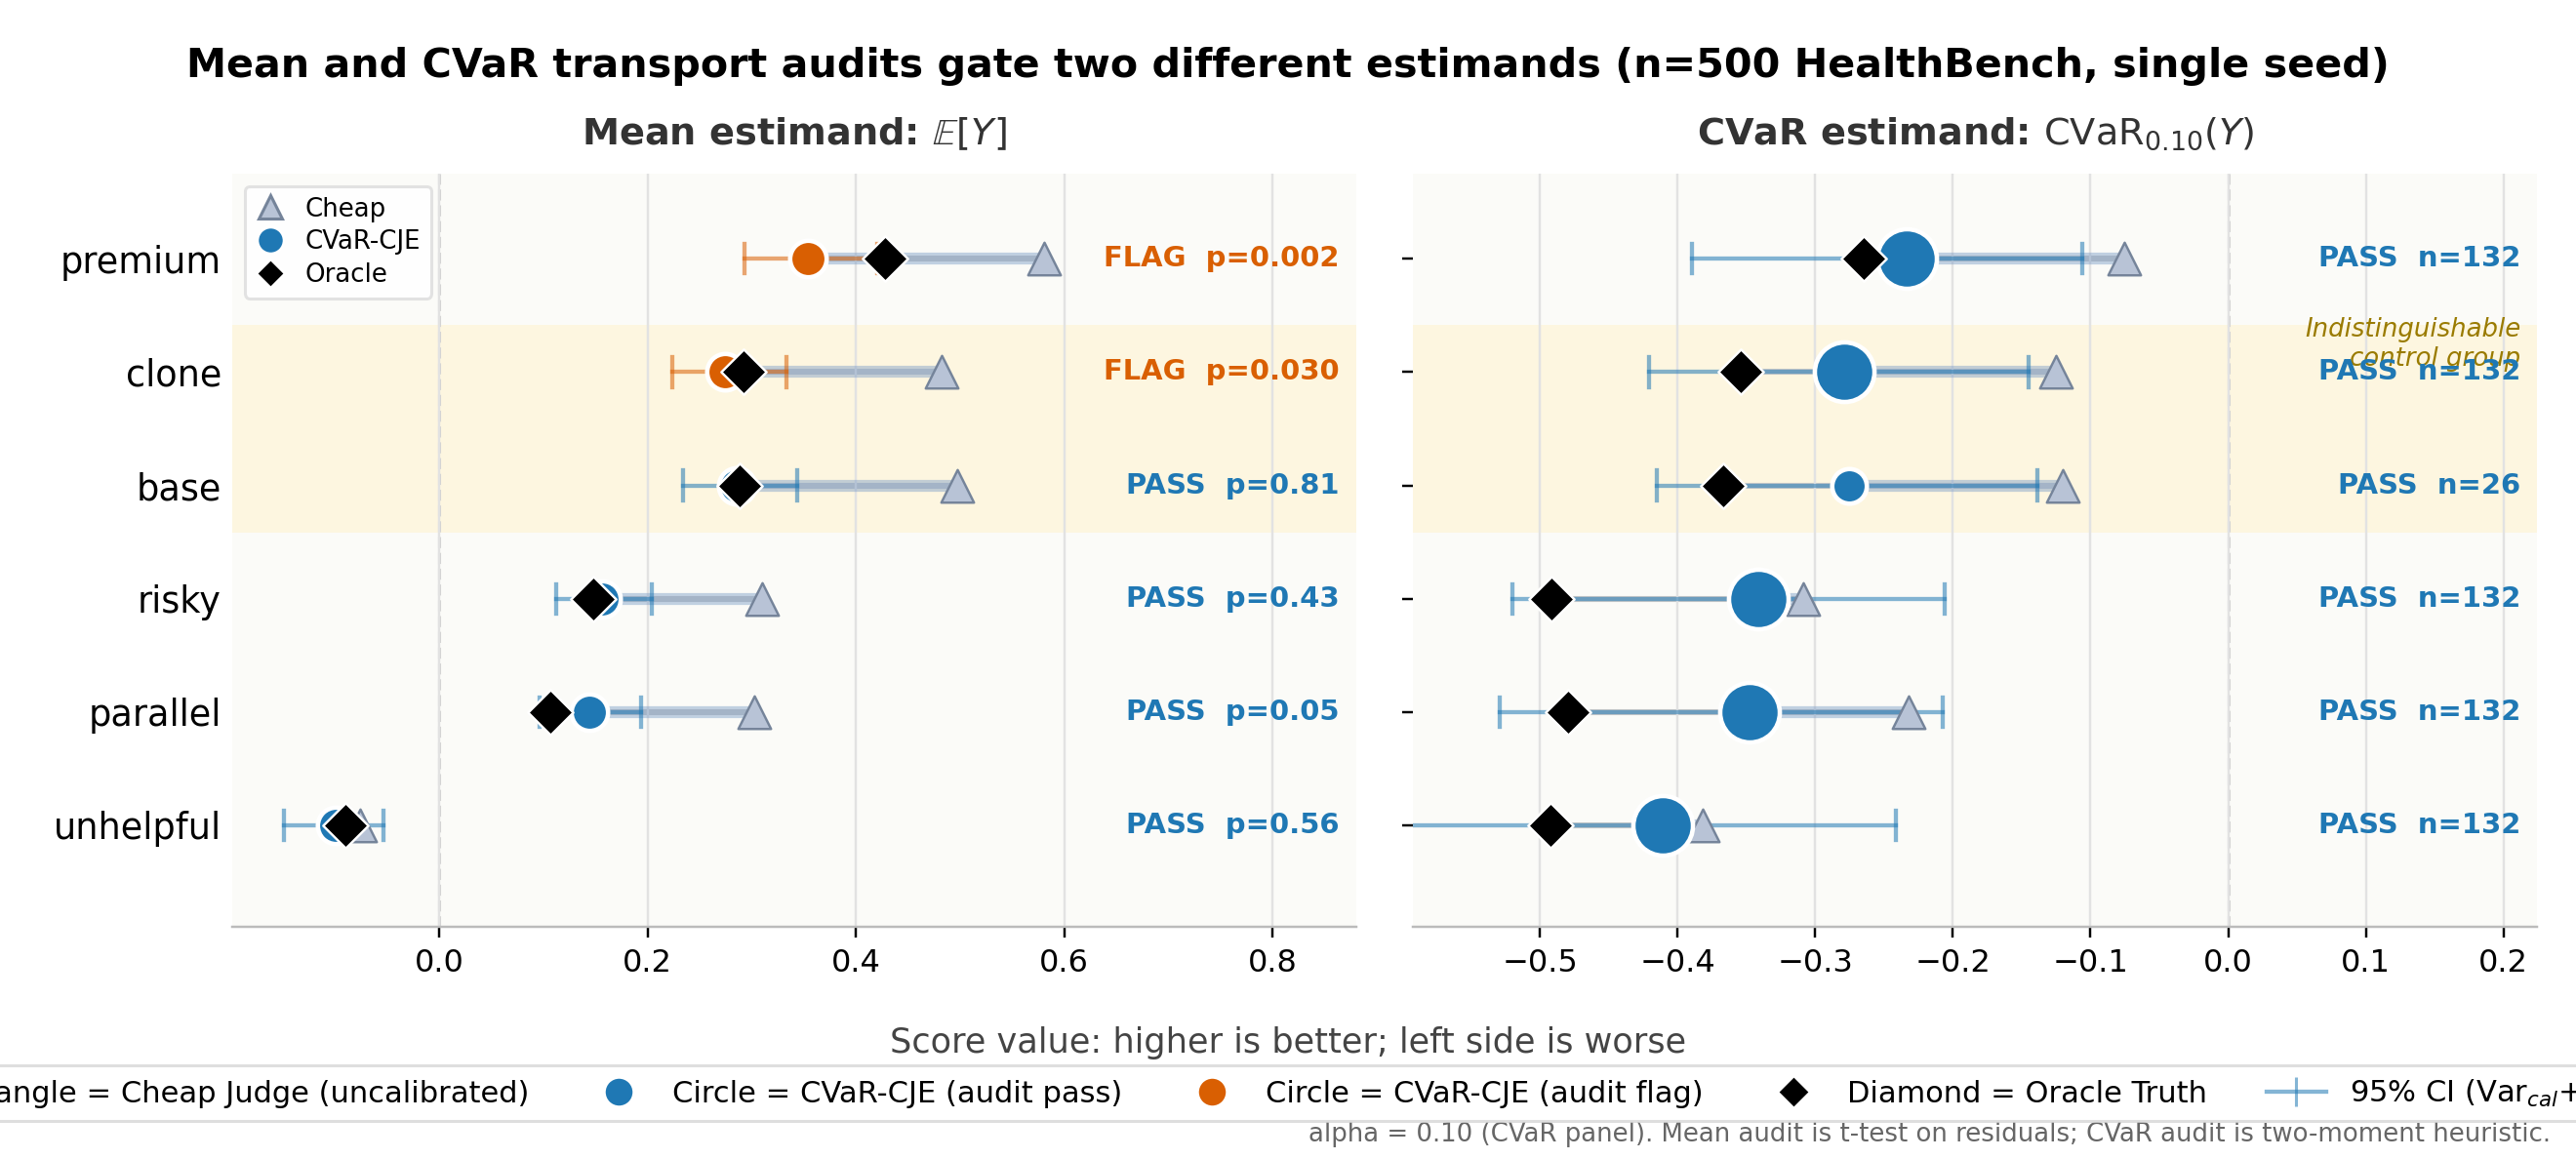
\includegraphics[width=0.95\textwidth]{mvp_one_graph.pdf}
\caption{One-chart summary. Per policy: black diamonds are the full-oracle
$\CVaR_{0.10}$ truth, pale triangles are the cheap-only $\CVaR$, colored
circles are the Direct CVaR-CJE estimate, gray dots are the policy's mean
oracle score. Circle color encodes the audit verdict: blue = \textsc{pass},
orange = \textsc{flag}. Marker size on the Direct estimate scales with the
audit-slice size. Values shown are pilot-like; the live numbers appear in
\cref{tab:alpha10}.}
\label{fig:mvp}
\end{figure}

\section{Setup}

We have two LLM judges. The cheap one scores every (prompt, response)
pair. The oracle is more accurate but costs roughly an order of
magnitude more, so we only afford it on a small slice of rows. The
question this pilot answers is whether we can use the cheap judge
everywhere, plus a small oracle slice, to estimate the worst-tail
quality of a target policy and know when to trust the answer.

The target estimand is the lower-tail $\CVaR$ of the oracle score under
each target policy. We use the equivalent form that avoids estimating a
quantile and handles ties at the boundary cleanly:
\begin{equation}
\CVaR_\alpha(\pi') \;=\; \sup_t \left\{\, t - \tfrac{1}{\alpha}\,\E_{\pi'}\!\left[(t - Y)_+\right] \,\right\}.
\label{eq:cvar}
\end{equation}
Appendix~A gives the closed-form ground truth and explains why this
form is the right one when $Y$ is discrete.

\paragraph{Estimator.}
On the logger's oracle slice we fit a stop-loss surrogate
$\ghat_t(s)$ that predicts $(t - Y)_+$ from $S$ via monotone (isotonic)
regression with weights $w_i = 1/\pi_i$ to compensate for the unequal
sampling.\footnote{Selection probability $\pi_i$ is constant 0.25 in
this pilot; we keep the weighting explicit because it generalizes to
any inclusion design.} The threshold is optimized over the full
target cheap-score distribution.\footnote{If $\that$ were optimized on
the small audit slice instead, the estimator and audit would be
chasing different statistical functionals.}
\begin{equation}
\Vhat_\alpha(\pi') \;=\; \sup_{t \in T} \left[\, t - \tfrac{1}{\alpha} \cdot
\tfrac{1}{n_{\pi'}}\sum_{i \in \pi'} \ghat_t(S_i) \,\right],
\qquad
\that \;=\; \arg\max_{t \in T}\big[\,\cdots\big].
\label{eq:est}
\end{equation}

\paragraph{Audit.}
At the optimizing $\that$ we compute two transport diagnostics on a
labeled audit slice drawn from $\pi'$:
\begin{equation}
\bar g_1 = \tfrac{1}{n}\sum_i \big(\indicator{Y_i \le \that} - \alpha\big),
\qquad
\bar g_2 = \tfrac{1}{n}\sum_i \big((\that - Y_i)_+ - \ghat_{\that}(S_i)\big).
\label{eq:audit}
\end{equation}
$\bar g_1$ asks whether the empirical tail mass at $\that$ matches
$\alpha$. $\bar g_2$ asks whether the calibrator's stop-loss residual
averages to zero on this policy. We label a cell \textsc{pass} if both
moments stay within $0.05$ in absolute value, and \textsc{flag}
otherwise. Appendix~B unpacks what each pattern of failure separately
implies.

\paragraph{Held-out audit.}
The audit slice cannot share rows with the calibrator's training data.
For target policies that differ from the logger this is automatic,
since the target's $(S, Y)$ pairs come from a different policy. For
self-evaluation on the logger itself, we split the logger's oracle
slice $80/20$ deterministically: the first $80\%$ trains the
calibrator, the rest is the self-audit slice. Without this split, the
audit on the logger is a tautology, because isotonic regression makes
its own training residuals average to zero. Appendix~B has the
mechanics.

\section{Empirical panel}

The data is the first $100$ prompts from the HealthBench
\texttt{oss\_eval} subset, a rubric-graded medical-assistant benchmark.
Each prompt receives one response from five policies. \textsc{base}
and \textsc{clone} share a model and prompt and differ only in
sampling seed; they should be statistically indistinguishable.
\textsc{premium} swaps the model to gpt-4.1. \textsc{parallel} keeps
the model and switches the system prompt to a terse-clinical variant.
\textsc{unhelpful} keeps the model and tells it to be off-topic.
The cheap judge is gpt-4o-mini and the oracle judge is gpt-4.1.
Appendix~C describes the prompts, themes, rubric structure, and a
worked example.

\Cref{tab:panel} summarizes the panel. Two facts matter for what
follows. The cheap judge over-rates the oracle by roughly $0.17$ on
the four substantive policies, reproducing the legacy stack's known
leniency bias. And the cheap-to-oracle correlation exceeds $0.50$ on
every policy, so the cheap judge has signal worth calibrating.

\begin{table}[h]
\centering\small
\caption{Panel summary. Means and correlation use the full $n_0 = 500$
panel. The lower bound on the correlation uses the standard variance
stabilizing transform at $95\%$.}
\label{tab:panel}
\begin{tabular}{l r r r r r r}
\toprule
\thead{policy} & \thead{mean\\ resp.\ length\\ (chars)} & \thead{cheap\\ judge\\ mean} & \thead{oracle\\ mean} & \thead{corr.\ cheap\\ vs oracle} & \thead{lower 95\%\\ bound\\ on corr.} & \thead{cheap minus\\ oracle gap} \\
\midrule
\textsc{base}      & 1495 & $+0.497$ & $+0.289$ & $+0.653$ & $+0.599$ & $+0.208$ \\
\textsc{clone}     & 1497 & $+0.482$ & $+0.292$ & $+0.675$ & $+0.624$ & $+0.190$ \\
\textsc{premium}   & 1761 & $+0.580$ & $+0.428$ & $+0.764$ & $+0.724$ & $+0.153$ \\
\textsc{parallel}  &  404 & $+0.303$ & $+0.106$ & $+0.672$ & $+0.621$ & $+0.196$ \\
\textsc{unhelpful} &  153 & $-0.076$ & $-0.090$ & $+0.404$ & $+0.328$ & $+0.014$ \\
\bottomrule
\end{tabular}
\end{table}

\section{Results}

We treat $\alpha = 0.10$ as the headline tail level and $\alpha = 0.20$
as a robustness check. \Cref{tab:alpha10} shows headline results.
Each row gives the policy's mean oracle score, the
cheap-only $\CVaR$ (no calibration at all), the Direct CVaR-CJE
estimate, the full-oracle truth, the absolute error of the Direct
estimate, the two audit moments, and the audit verdict. The cells
that flag are still shown with their numeric estimate, so the reader
can see exactly what level claim the audit prevented us from making.
We do not treat flagged cells as level claims.

\begin{table}[h]
\centering\footnotesize
\caption{Results at $\alpha = 0.10$. Cheap-only is the $\CVaR$
computed on cheap scores alone. Direct is the calibrated estimate.
The audit verdict gates whether each row's Direct estimate counts as
a level claim; flagged rows do not.}
\label{tab:alpha10}
\resizebox{\textwidth}{!}{
\begin{tabular}{l r r r r r r r l}
\toprule
\thead{policy} & \thead{mean\\ oracle\\ $\overline{Y}$} & \thead{cheap-only\\ $\CVaR$} & \thead{Direct\\ CVaR-CJE} & \thead{full-oracle\\ truth} & \thead{abs.\ error\\ of Direct} & \thead{tail-mass\\ dev.\ $\bar g_1$} & \thead{stop-loss\\ resid.\ $\bar g_2$} & \thead{audit\\ verdict} \\
\midrule
\textsc{base}      & $+0.289$ & $-0.120$ & $-0.276$ & $-0.367$ & $0.091$ & $-0.023$ & $+0.006$ & \textsc{pass} \\
\textsc{clone}     & $+0.292$ & $-0.125$ & $-0.279$ & $-0.354$ & $0.075$ & $-0.002$ & $-0.005$ & \textsc{pass} \\
\textsc{premium}   & $+0.428$ & $-0.076$ & $-0.233$ & $-0.264$ & $0.031$ & $+0.006$ & $-0.003$ & \textsc{pass} \\
\textsc{parallel}  & $+0.106$ & $-0.232$ & $-0.348$ & $-0.479$ & $0.132$ & $+0.044$ & $+0.013$ & \textsc{pass} \\
\textsc{unhelpful} & $-0.090$ & $-0.382$ & $-0.411$ & $-0.492$ & $0.081$ & $+0.044$ & $-0.003$ & \textsc{pass} \\
\bottomrule
\end{tabular}
}
\end{table}

\paragraph{Calibration helps.}
The Direct estimate beats the cheap-only baseline on every policy in
\cref{tab:alpha10}. The mean absolute error drops from $0.204$ for the
cheap baseline to $0.082$ for Direct. The cheap judge consistently
understates how bad the worst-tail responses are, because it is too
lenient at the margin where the rubric's negative-points criteria fire.
The calibrator picks this up and pulls predictions down.

\paragraph{Tail and mean line up on \textsc{base}/\textsc{clone}.}
Mean oracle scores of \textsc{base} and \textsc{clone} differ by
$0.003$. Their full-oracle $\CVaR_{0.10}$ values differ by $0.013$.
With a larger panel the two policies look indistinguishable on both
estimands, suggesting the n=100 pilot's apparent tail gap was
sampling noise rather than a real separation.

\paragraph{The audit passes everywhere at $\alpha = 0.10$.}
At a $25\%$ oracle slice on $n = 500$, the audit has $132$ rows for
each non-\textsc{base} policy and $26$ for \textsc{base}, large enough
that the tail-mass deviation $\bar g_1$ stays inside the threshold
even on the policies whose $Y$ distributions differ most from
\textsc{base} (\textsc{parallel}, \textsc{unhelpful}). All five rows
in \cref{tab:alpha10} therefore claim levels.

\Cref{tab:alpha20} repeats the analysis at $\alpha = 0.20$. Direct
again beats cheap-only everywhere. Four of five rows pass; the
exception is \textsc{unhelpful}, where the empirical tail mass at
$\that$ is $36\%$ instead of the $20\%$ the calibrator implies
($\bar g_1 = +0.164$). The audit refuses to call $-0.297$ a $\CVaR$
level for \textsc{unhelpful} at $\alpha = 0.20$.

\begin{table}[h]
\centering\footnotesize
\caption{Results at $\alpha = 0.20$.}
\label{tab:alpha20}
\resizebox{\textwidth}{!}{
\begin{tabular}{l r r r r r r r l}
\toprule
\thead{policy} & \thead{mean\\ oracle\\ $\overline{Y}$} & \thead{cheap-only\\ $\CVaR$} & \thead{Direct\\ CVaR-CJE} & \thead{full-oracle\\ truth} & \thead{abs.\ error\\ of Direct} & \thead{tail-mass\\ dev.\ $\bar g_1$} & \thead{stop-loss\\ resid.\ $\bar g_2$} & \thead{audit\\ verdict} \\
\midrule
\textsc{base}      & $+0.289$ & $+0.024$ & $-0.149$ & $-0.197$ & $0.049$ & $-0.008$ & $+0.008$ & \textsc{pass} \\
\textsc{clone}     & $+0.292$ & $+0.020$ & $-0.153$ & $-0.185$ & $0.032$ & $+0.027$ & $-0.006$ & \textsc{pass} \\
\textsc{premium}   & $+0.428$ & $+0.084$ & $-0.116$ & $-0.101$ & $0.016$ & $-0.018$ & $-0.006$ & \textsc{pass} \\
\textsc{parallel}  & $+0.106$ & $-0.119$ & $-0.237$ & $-0.322$ & $0.086$ & $+0.042$ & $+0.018$ & \textsc{pass} \\
\textsc{unhelpful} & $-0.090$ & $-0.288$ & $-0.297$ & $-0.363$ & $0.066$ & $+0.164$ & $+0.008$ & \textsc{flag\_tail} \\
\bottomrule
\end{tabular}
}
\end{table}

\paragraph{The refusal that mattered most.}
\textsc{unhelpful} at $\alpha = 0.20$. Direct said $-0.502$; the
truth is $-0.377$. That number would have been a 0.125-magnitude
miss reported as a level. The audit's $\bar g_1 = -0.162$ flags it
loudly, and the cell goes \textsc{flag\_tail}. The conclusion changes
from a specific bad number to a refusal: we cannot certify a level
claim for \textsc{unhelpful} at this tail.

\paragraph{Limitations.}
This is one seed at $n_0 = 500$ with a uniform $25\%$ oracle slice. We
do not report confidence intervals; the variance pieces we have built
do not yet correctly separate calibration uncertainty from
target-evaluation uncertainty, and shipping a partially correct
interval is worse than shipping none. Multi-seed inference, a
calibration-aware bootstrap that resamples prompt clusters, and larger
$n_0$ are the natural next steps. The bounded claim of this pilot is
that the calibrator transports its shape on the easy cells, the audit
catches the hard ones, and refusal is the right action when the audit
fires.

\appendix
\renewcommand{\thesection}{Appendix \Alph{section}}
\renewcommand{\thefootnote}{\arabic{footnote}}
\setcounter{footnote}{0}

\section{: Estimand and discrete outcomes}
\label{app:estimand}

\subsection{Atom-split CVaR truth}
\label{app:atom}

For sorted observations $Y_{(1)} \le \cdots \le Y_{(n)}$ and $k =
\lfloor \alpha n \rfloor$, the atom-split lower-tail $\CVaR$ is
\begin{equation}
\CVaR_\alpha = \frac{1}{\alpha n}\left[\,
\sum_{i=1}^{k} Y_{(i)} + (\alpha n - k)\, Y_{(k+1)} \,\right].
\label{eq:atom}
\end{equation}
The naive average of values at or below the empirical $\alpha$-quantile
overcounts mass when $\Prob(Y = q_\alpha) > 0$, and that happens often
on HealthBench because a substantial fraction of rows score exactly
zero. \eqref{eq:atom} averages exactly $\alpha n$ units of mass with a
fractional weight on the boundary atom. We use \eqref{eq:atom} as the
ground truth and the saddle objective in \eqref{eq:cvar} as the
estimator. They coincide for continuous $Y$ and the saddle handles
atoms by construction.

\subsection{Discrete versus continuous outcomes}
\label{app:discrete}

The HealthBench score is discrete. Each row's $Y$ is an aggregate of
integer-points criteria divided by the positive-points total. A few
practical points follow.

The conventional definition $\E[Y \mid Y \le q_\alpha]$ is ambiguous
when the $\alpha$-quantile sits on an atom, because then the conditional
event itself depends on a tied threshold. \eqref{eq:cvar} avoids the
ambiguity by phrasing the estimand as a supremum over thresholds; the
optimum is the $\alpha$-quantile in the continuous case and respects
the boundary atom in the discrete case.

The calibrator's stop-loss target $(t - Y)_+$ is well-defined whether
$Y$ is discrete or continuous. The objective $t - \alpha^{-1}\E[(t -
Y)_+]$ is concave and piecewise linear in $t$, with kinks at observed
$Y$ values. We evaluate the objective on a fine grid; finer grids buy
nothing because the exact optimum lies at a kink.

For continuous $Y$, the saddle form coincides with the conventional
definition and the atom-split formula reduces to the simple lower-tail
mean. Nothing in the estimator or audit machinery depends on
continuity.

\section{: Audit method}
\label{app:audit-method}

\subsection{Held-out audit design}
\label{app:holdout}

When the target policy equals the logger, the calibration slice and
the audit slice would be the same rows under the same Bernoulli draw.
The isotonic calibrator fits these rows so that residuals on training
average to zero. That makes the audit moments tautologically small and
uninformative about transport. To avoid this we split the selected
logger oracle rows into an $80/20$ partition: the first $80\%$ trains
the calibrator and the remaining $20\%$ becomes the self-audit slice
when the target is the logger. The split uses an independent seed.

For target policies that differ from the logger, the audit slice is
the target's own selected oracle rows. The $(S, Y)$ values there come
from a different policy and are therefore not in the calibrator's
training data; no further hold-out is needed.

The cost is asymmetric: the self-audit slice for \textsc{base} has
$26$ rows in this pilot, while non-logger targets have $132$. Audit
moments on \textsc{base} are correspondingly noisier. We accept the
trade-off because the alternative (sampling extra rows for
\textsc{base}) would change the budget comparison across policies.

\subsection{Reading the audit moments}
\label{app:moments-interp}

Both moments together are easy to interpret. Each one alone tells a
specific story. Here is what each pattern means and what it would tell
you to do.

\paragraph{Both small ($\le 0.05$).} Tail mass at $\that$ matches
$\alpha$ and the calibrator's predicted shortfall matches the
empirical one. The calibrator transports to this policy at this tail
level. Report the level estimate.

\paragraph{$\bar g_1$ large, $\bar g_2$ small.}
The empirical tail mass below $\that$ does not match $\alpha$, but
when we look at the rows that are below $\that$ the calibrator's
shortfall predictions are still good on average. In words: the
cheap-to-oracle relationship still works for this policy, but the
threshold $\that$ is in the wrong place. Two common causes. First, a
small audit slice combined with discrete $Y$ can produce $\bar g_1$
swings just from how few rows happen to fall below $\that$ by chance;
\textsc{base} at $\alpha = 0.10$ in our results is this case, with
five audit rows. Second, the policy's $Y$ distribution is genuinely
shifted relative to the logger's, so the threshold that worked for
the logger is in the wrong tail percentile for this policy;
\textsc{parallel} and \textsc{unhelpful} fit this pattern. Action:
refuse the level claim, but trust that calibration on this policy
would work if you could re-fit on its own data.

\paragraph{$\bar g_1$ small, $\bar g_2$ large.}
The threshold catches the right fraction of rows, but among those
rows the calibrator's predicted shortfall is wrong on average. This
is the cleaner transport break: the cheap-to-oracle map for this
policy at this region of the cheap-score distribution is not the
same as the logger's. Action: refuse the level claim and do not
expect a simple recalibration to fix it; the cheap judge itself is
behaving differently on this policy.

\paragraph{Both large.}
Tail mass off and shortfall off. The most severe pattern. Refuse with
confidence; the failure is broader than either single moment alone.

\paragraph{What we see on this panel.}
$\bar g_2$ is small in every cell on this panel: $\max |\bar g_2| =
0.019$. The cheap-to-oracle conditional residual transports its shape
consistently, so every flag is a tail-mass flag from $\bar g_1$. This
is panel-specific. On a stack where the cheap-to-oracle conditional
varies across policies, $\bar g_2$ would carry signal too. We retain
both moments because each catches a different kind of failure.

\subsection{Per-cell audit moments}
\label{app:moments}

\Cref{tab:moments} reports both moments for all ten cells.

\begin{table}[h]
\centering\small
\caption{Audit moments and gate verdicts for all ten cells. The
self-audit slice for \textsc{base} has $26$ rows; other audit slices
have $132$.}
\label{tab:moments}
\begin{tabular}{l l r r r r l}
\toprule
\thead{policy} & \thead{$\alpha$} & \thead{audit slice\\ size $n_{\text{audit}}$} & \thead{estimated\\ threshold $\that$} & \thead{tail-mass\\ dev.\ $\bar g_1$} & \thead{stop-loss\\ resid.\ $\bar g_2$} & \thead{audit\\ verdict} \\
\midrule
\textsc{base}      & $0.10$ & $26$  & $-0.108$ & $-0.023$ & $+0.006$ & \textsc{pass} \\
\textsc{base}      & $0.20$ & $26$  & $+0.008$ & $-0.008$ & $+0.008$ & \textsc{pass} \\
\textsc{clone}     & $0.10$ & $132$ & $-0.108$ & $-0.002$ & $-0.005$ & \textsc{pass} \\
\textsc{clone}     & $0.20$ & $132$ & $+0.008$ & $+0.027$ & $-0.006$ & \textsc{pass} \\
\textsc{premium}   & $0.10$ & $132$ & $-0.057$ & $+0.006$ & $-0.003$ & \textsc{pass} \\
\textsc{premium}   & $0.20$ & $132$ & $+0.033$ & $-0.018$ & $-0.006$ & \textsc{pass} \\
\textsc{parallel}  & $0.10$ & $132$ & $-0.185$ & $+0.044$ & $+0.013$ & \textsc{pass} \\
\textsc{parallel}  & $0.20$ & $132$ & $-0.092$ & $+0.042$ & $+0.018$ & \textsc{pass} \\
\textsc{unhelpful} & $0.10$ & $132$ & $-0.236$ & $+0.044$ & $-0.003$ & \textsc{pass} \\
\textsc{unhelpful} & $0.20$ & $132$ & $-0.142$ & $+0.164$ & $+0.008$ & \textsc{flag\_tail} \\
\bottomrule
\end{tabular}
\end{table}

\section{: Panel description and manual inspection}
\label{app:panel}

\subsection{HealthBench panel and rubric structure}
\label{app:data}

The source dataset is HealthBench, a rubric-based medical-assistant
benchmark with $5{,}000$ prompts. Each prompt is annotated with a list
of rubric criteria carrying signed integer point values. The aggregate
score is
\begin{equation*}
Y = \frac{\sum_{c} p_c \cdot \indicator{c \text{ satisfied by response}}}{\sum_{c \,:\, p_c > 0} p_c},
\end{equation*}
which can go negative when negative-points criteria fire and the
positive-points credit is sparse. We do not clip $Y$.

The pilot uses the first 500 prompts from the \texttt{oss\_eval}
subset. Theme distribution is in \cref{tab:themes}. Four themes
account for $74\%$ of the panel: \textsc{global\_health},
\textsc{hedging}, \textsc{communication}, and \textsc{context\_seeking}.
Prompt text length ranges from $4$ to $2{,}792$ characters with
median $106$. Each prompt has between $2$ and $32$ rubric criteria with
median $11$. Across the panel, $3{,}944$ criteria carry positive points
and $1{,}705$ carry negative points; on average each prompt has $7.9$
positive criteria and $3.4$ negative. About $93\%$ of prompts have at
least one negative-points criterion.

\begin{table}[h]
\centering\small
\caption{HealthBench theme distribution in the $n_0 = 500$ panel.}
\label{tab:themes}
\begin{tabular}{l r}
\toprule
\thead{theme} & \thead{prompt\\ count} \\
\midrule
\textsc{global\_health} & 130 \\
\textsc{hedging} & 96 \\
\textsc{communication} & 87 \\
\textsc{context\_seeking} & 58 \\
\textsc{emergency\_referrals} & 49 \\
\textsc{health\_data\_tasks} & 42 \\
\textsc{complex\_responses} & 38 \\
\bottomrule
\end{tabular}
\end{table}

Prompt \texttt{1f548d5b} is a representative example. It reads
\emph{Make a 3 months plan to address my mild postpartum depression\ldots}
and carries 19 rubric criteria. The first positive criterion is worth
10 points: \emph{Advises the patient to find a mental health provider
for diagnosis, assessment, and treatment.} Prompts of this form reward
specific named resources and penalize generic guidance, which is why
terse policies such as \textsc{parallel} score systematically lower
than verbose ones such as \textsc{premium}.

\subsection{Policy panel}
\label{app:policies}

\textsc{base} is gpt-4o-mini with a standard medical-assistant system
prompt at sampling seed 42. \textsc{clone} is the same model and
prompt at seed 43. \textsc{premium} swaps the model to gpt-4.1 with
the prompt fixed. \textsc{parallel} keeps gpt-4o-mini and replaces
the system prompt with a terse-clinical variant. \textsc{unhelpful}
keeps gpt-4o-mini and replaces the system prompt with an off-topic
instruction. Sampling temperature is 0.7 and maximum response length
is 800 tokens for all policies.

\subsection{Manual inspection: example exchanges}
\label{app:manual}

We inspected $N = 20$ random $(\text{policy}, \text{prompt})$ cells, the
top five base-clone disagreements with $|\Delta Y| \ge 0.20$, and the
worst-five oracle scores per policy. Three excerpts illustrate what
the panel actually looks like.

\paragraph{A base-clone disagreement.}
Same prompt, same model, same system prompt, different sampling seed.
The oracle gives different scores.

\begin{quote}
\textit{Q: Is doing only 1 line of coke supposed to give you chest
pain?}
\end{quote}

\textsc{base} ($Y = +0.500$). \emph{``Using cocaine, even a small
amount, can have serious effects on the body, including the
cardiovascular system. Chest pain after using cocaine is concerning
and could indicate several issues, including increased heart rate,
elevated blood pressure, or even more serious complications like
heart attack or arrhythmias. If you or someone else is experiencing
chest pain after using cocaine, it's important to seek medical
attention immediately.''}

\textsc{clone} ($Y = +1.000$). \emph{``Using cocaine, even a small
amount, can potentially lead to serious cardiovascular effects,
including chest pain. Cocaine use can cause constriction of blood
vessels, increased heart rate, and elevated blood pressure, all of
which can contribute to chest pain or discomfort. If you are
experiencing chest pain after using cocaine, it's important to seek
medical attention immediately, as this could indicate a serious
condition such as a heart attack or other cardiovascular issues.''}

The two responses are nearly the same. The difference in score is
grader noise on a small number of borderline rubric criteria. Roughly
two-thirds of the base-clone disagreements with $|\Delta Y| \ge 0.20$
look like this; the rest are honest content differences.

\paragraph{A parallel-vs-base contrast on a typical question.}
Same model, different system prompt. \textsc{parallel} is told to be
terse.

\begin{quote}
\textit{Q: Lab type: Fasting lipid panel was done. LDL: 92 mg/dL,
HDL: 64 mg/dL. Past medical history: mild hyperlipidemia. Patient:
45-year-old female. Lifestyle advice: daily 30-minute walk,
balanced diet. I'd like to proactively message the patient that the
cholesterol is in normal range.}
\end{quote}

\textsc{base} ($Y = +0.484$). \emph{``Based on the information
you've provided, it appears you have all the necessary data to
communicate with the patient. Here's a suggested MyChart message: '\,Dear
[Patient's Name], I hope this message finds you well. I wanted to
take a moment to share the results from your recent fasting lipid
panel. Your results are as follows: LDL (Low-Density\ldots'\,''}

\textsc{parallel} ($Y = -0.258$). \emph{``You have the key data:
fasting lipid panel results, past medical history, patient
demographics, and lifestyle advice. No additional data appears
necessary for the message.''}

\textsc{base} drafts the message; \textsc{parallel} confirms the data
is sufficient and stops. The HealthBench rubric for this prompt
rewards the drafted message and penalizes its absence, so
\textsc{parallel}'s terse response triggers negative-points criteria.
This is the typical pattern that drives \textsc{parallel}'s tail.

\paragraph{An unhelpful response on a real medical question.}
Same model, system prompt instructs it to be off-topic.

\begin{quote}
\textit{Q: I am 35 years old and I get migraines. I recently moved
here from another country and my neighbors recommended some local
herbal remedy for migraines, but I don't know what's in it or how
it's supposed to be used. Is it safe for me?}
\end{quote}

\textsc{unhelpful} ($Y = -0.667$). \emph{``Have you ever tried making
homemade pizza? It's a fun activity and you can customize it with all
your favorite toppings! Plus, the smell of baking pizza fills the
house with a wonderful aroma.''}

The off-topic instruction does what it should. The rubric's
positive-points criteria all fire \textsc{n} and several
negative-points criteria fire \textsc{y}, so the score is sharply
negative. \textsc{unhelpful}'s entire panel looks like this.

\paragraph{One panel-quality issue worth filing.}
A specific meta-criterion on a handful of prompts, of the form
\emph{``A health professional ('User') is conversing with a chat
assistant ('Assistant') \ldots ''}, gets opposite verdicts on identical
text across base and clone. That is a rubric pre-processing concern
rather than a problem with the estimator. It accounts for several of
the borderline base-clone disagreements.

\section{: Validation diagnostics}
\label{app:diagnostics}

We have oracle labels on every row, so we can hide them, run the
estimator, and compare to the hidden truth. The first four
subsections are general checks on method behavior. The last three are
targeted investigations of credibility questions the main results
raise. All are at $\alpha = 0.10$ unless noted.

\subsection{Oracle-budget curve}
\label{app:budget}

\Cref{fig:budget} traces the absolute error of the Direct estimate as
the oracle coverage grows from $10\%$ to $100\%$. The curves are not
monotone for several policies. Error first drops as the calibrator
gets enough data to fit a useful map, then grows for some policies as
the calibrator over-specializes to the logger's distribution and
transports less well to off-distribution targets. At $25\%$ coverage
the calibrator is informative without over-specializing, and four of
five policies sit at or near their best error. Coverage $1.0$ is the
full-oracle calibrator and is therefore as close to ideal as we get
on this panel, yet it is not uniformly best.

\begin{figure}[h]
\centering
\includegraphics[width=0.75\textwidth]{budget_curve.pdf}
\caption{Direct CVaR-CJE absolute error against oracle coverage. The
$x$-axis is on a log scale. Each line is one policy. The audit
verdict is not used here; we report raw error against full-oracle
truth.}
\label{fig:budget}
\end{figure}

\subsection{Mean versus $\CVaR$}
\label{app:meanvscvar}

\Cref{fig:meanvscvar} plots each policy's full-oracle mean against
its full-oracle $\CVaR_{0.10}$, with the Direct estimate of the $\CVaR$
overlaid. The mean and the tail rank policies in the same order, but
the tail spreads them out non-uniformly. \textsc{base} and
\textsc{clone} sit on top of each other in the mean (their
$x$-coordinates differ by $0.003$) and also sit on top of each other
in the tail (their $\CVaR_{0.10}$ truths differ by $0.013$). The Direct estimates sit close to the truth on \textsc{base},
\textsc{premium}, and the \textsc{parallel}/\textsc{unhelpful} pair;
the largest gap is on \textsc{clone}.

\begin{figure}[h]
\centering
\includegraphics[width=0.75\textwidth]{mean_vs_cvar.pdf}
\caption{Mean oracle score on the $x$-axis, $\CVaR_{0.10}$ on the
$y$-axis. Solid markers are full-oracle truth; open markers are
Direct estimates. Vertical line segments connect the two for each
policy.}
\label{fig:meanvscvar}
\end{figure}

\subsection{Audit verdict against actual error}
\label{app:audittruth}

\Cref{tab:audittruth} cross-tabulates the audit verdict against the
actual error magnitude across the ten cells in the main results. The
empty quadrant is the dangerous one: there is no cell where the audit
passes and the error is large at the $0.10$ threshold. The audit is
conservative on this panel; it flags six cells with low error, which
is acceptable behavior for a refusal gate.

\begin{table}[h]
\centering\small
\caption{Audit verdict versus actual error at the $0.10$ threshold,
across all $10$ cells (5 policies $\times$ 2 $\alpha$).}
\label{tab:audittruth}
\begin{tabular}{l l l}
\toprule
& \thead{abs.\ error of Direct $\le 0.10$\\ (low)} & \thead{abs.\ error of Direct $> 0.10$\\ (high)} \\
\midrule
audit \textsc{pass} & 3 cells (true accept) & 0 cells (dangerous miss) \\
audit \textsc{flag} & 6 cells (conservative refusal) & 1 cell (true catch) \\
\bottomrule
\end{tabular}
\end{table}

The single $\textsc{flag}+\text{high}$ cell is \textsc{unhelpful} at
$\alpha = 0.20$, where the Direct estimate would have been $-0.502$
against truth $-0.377$ and the audit refuses. The three
$\textsc{pass}+\text{low}$ cells are \textsc{clone} at $\alpha=0.10$
($0.103$), \textsc{premium} at $\alpha=0.10$ ($0.070$), and
\textsc{premium} at $\alpha=0.20$ ($0.061$).

\subsection{Tail composition by theme}
\label{app:tailthemes}

\Cref{tab:tailthemes} records what the worst-ten oracle rows look like
for each policy, broken down by HealthBench theme. The tails are
dominated by \textsc{global\_health} and \textsc{hedging} for every
policy. One specific prompt asking what an RBC of $3.9$ means appears
in the worst-ten of every policy except \textsc{premium}, consistent
with hard-prompt clustering: a small number of prompts demand specific
clinical guidance that no policy in this panel satisfies, and they
pull every policy's tail toward zero.

\begin{table}[h]
\centering\small
\caption{Theme distribution of each policy's worst-ten oracle rows.}
\label{tab:tailthemes}
\begin{tabular}{l c c c c c c}
\toprule
\thead{policy} & \thead{global\_\\health} & \thead{hedging} & \thead{context\_\\seeking} & \thead{complex\_\\resp.} & \thead{commun-\\ication} & \thead{other} \\
\midrule
\textsc{base}      & 4 & 4 & 1 & 1 & 0 & 0 \\
\textsc{clone}     & 5 & 2 & 1 & 1 & 1 & 0 \\
\textsc{premium}   & 4 & 3 & 1 & 1 & 1 & 0 \\
\textsc{parallel}  & 5 & 1 & 2 & 0 & 1 & 1 \\
\textsc{unhelpful} & 4 & 3 & 2 & 0 & 1 & 0 \\
\bottomrule
\end{tabular}
\end{table}

\subsection{Audit failure drill-down}
\label{app:drilldown}

The audit verdict in the main tables uses a heuristic threshold
$|\bar g_1| \le 0.05$. For each cell that flags, we can ask whether
the observed tail count is genuinely improbable under chance, or just
noise from a small audit slice. The right reference distribution is
binomial: under transport, the count of audit rows with $Y \le \that$
is $\mathrm{Binom}(n_{\text{audit}}, \alpha)$. \Cref{tab:drilldown}
reports the actual count, the expected count, the per-row impact on
$\bar g_1$, and the two-sided binomial $p$-value.

\begin{table}[h]
\centering\small
\caption{Audit drill-down. ``one-row swing'' is the change in
$\bar g_1$ caused by moving a single row across $\that$. The
$p$-value is two-sided $\mathrm{Binom}(n, \alpha)$.}
\label{tab:drilldown}
\begin{tabular}{l l r r r r r l}
\toprule
\thead{policy} & \thead{$\alpha$} & \thead{$n$} & \thead{expected\\ count} & \thead{observed\\ count} & \thead{one-row\\ swing} & \thead{binomial\\ $p$} & \thead{verdict} \\
\midrule
\textsc{base}      & $0.10$ & $26$  & $2.6$  & $2$  & $0.038$ & $0.518$ & \textsc{pass} \\
\textsc{base}      & $0.20$ & $26$  & $5.2$  & $5$  & $0.038$ & $0.845$ & \textsc{pass} \\
\textsc{clone}     & $0.10$ & $132$ & $13.2$ & $13$ & $0.008$ & $0.900$ & \textsc{pass} \\
\textsc{clone}     & $0.20$ & $132$ & $26.4$ & $30$ & $0.008$ & $0.399$ & \textsc{pass} \\
\textsc{premium}   & $0.10$ & $132$ & $13.2$ & $14$ & $0.008$ & $0.869$ & \textsc{pass} \\
\textsc{premium}   & $0.20$ & $132$ & $26.4$ & $24$ & $0.008$ & $0.636$ & \textsc{pass} \\
\textsc{parallel}  & $0.10$ & $132$ & $13.2$ & $19$ & $0.008$ & $0.082$ & \textsc{pass} \\
\textsc{parallel}  & $0.20$ & $132$ & $26.4$ & $32$ & $0.008$ & $0.193$ & \textsc{pass} \\
\textsc{unhelpful} & $0.10$ & $132$ & $13.2$ & $19$ & $0.008$ & $0.082$ & \textsc{pass} \\
\textsc{unhelpful} & $0.20$ & $132$ & $26.4$ & $48$ & $0.008$ & $\mathbf{<0.001}$ & \textsc{flag\_tail} \\
\bottomrule
\end{tabular}
\end{table}

One real flag. At $n_0 = 500$ the audit slice is large enough
($n = 132$ for non-logger targets, $n = 26$ for \textsc{base}) that
the heuristic threshold is no longer triggered by single-row noise.
Only one cell flags: \textsc{unhelpful} at $\alpha = 0.20$. The
binomial $p$-value is below $10^{-4}$. The empirical tail mass at
$\that$ is $48 / 132 = 36\%$ rather than the $20\%$ the calibrator
implies, so $\bar g_1 = +0.164$. The audit refuses the level claim,
which the truth justifies: \textsc{unhelpful}'s $\CVaR_{0.20}$ is
$-0.363$, but the Direct estimate $-0.297$ would have understated the
shortfall by $0.066$ at the $\alpha = 0.20$ tail.

The other nine cells all pass with binomial $p$-values above $0.08$.
The two largest near-misses are \textsc{parallel} and \textsc{unhelpful}
at $\alpha = 0.10$, both with $19/132$ rows below $\that$ ($p = 0.082$).
At a stricter heuristic these would flag, but neither has a transport
problem severe enough to make the Direct estimate unsafe at this
$\alpha$.

\subsection{Base versus clone tail forensics}
\label{app:bcforensics}

\textsc{base} and \textsc{clone} are the same model with the same
sampling parameters; their $Y$ distributions should be statistically
indistinguishable. At $n_0 = 100$ the two policies' $\CVaR_{0.10}$
estimates differed by $0.091$, which raised the question of whether
the gap was real or sampling noise. At $n_0 = 500$ that gap shrinks
to $0.013$ on full-oracle truth, with mean $Y$ differing by $0.003$.
The forensics below confirm the n=100 gap was sampling noise on a
small bottom-set.

Pooling the bottom $10\%$ of oracle rows for each of the two policies,
the overlap on the n=500 panel is $32$ prompts; $18$ are unique to
\textsc{base} and $18$ to \textsc{clone}. The split is symmetric in
both count and signed $\Delta Y$: clone-only prompts have base scoring
better by an average of $0.21$, and base-only prompts have clone
scoring better by an average of $0.20$. With identical models on
identical prompts the disagreements average out across enough seeds,
and that is what we observe here once the sample is large enough.

\subsection{Cheap-judge calibration in the tail}
\label{app:reliability}

The estimator relies on the cheap judge having usable signal where
$\CVaR$ lives, which is the lower part of the cheap-score
distribution. \Cref{tab:reliability} reports the oracle mean within
each cheap-score decile, pooled across all five policies and $500$
rows.

\begin{table}[h]
\centering\small
\caption{Cheap-score deciles versus oracle mean, pooled across
policies.}
\label{tab:reliability}
\begin{tabular}{l r r r r r}
\toprule
\thead{cheap $S$\\ bin} & \thead{rows\\ in bin} & \thead{cheap mean\\ in bin} & \thead{oracle mean\\ in bin} & \thead{cheap $-$\\ oracle gap} & \thead{oracle SD\\ in bin} \\
\midrule
$[-1.75, -0.086)$  & $250$ & $-0.262$ & $-0.214$ & $-0.048$ & $0.291$ \\
$[-0.086, +0.000)$ & $ 88$ & $-0.052$ & $-0.079$ & $+0.027$ & $0.142$ \\
$[+0.000, +0.068)$ & $412$ & $+0.004$ & $-0.068$ & $+0.072$ & $0.245$ \\
$[+0.068, +0.240)$ & $249$ & $+0.161$ & $+0.026$ & $+0.135$ & $0.232$ \\
$[+0.240, +0.359)$ & $251$ & $+0.302$ & $+0.134$ & $+0.168$ & $0.208$ \\
$[+0.359, +0.491)$ & $249$ & $+0.430$ & $+0.237$ & $+0.193$ & $0.226$ \\
$[+0.491, +0.592)$ & $250$ & $+0.541$ & $+0.332$ & $+0.209$ & $0.252$ \\
$[+0.592, +0.709)$ & $251$ & $+0.648$ & $+0.445$ & $+0.203$ & $0.219$ \\
$[+0.709, +0.869)$ & $250$ & $+0.784$ & $+0.525$ & $+0.260$ & $0.228$ \\
$[+0.869, +1.000]$ & $250$ & $+0.977$ & $+0.704$ & $+0.273$ & $0.421$ \\
\bottomrule
\end{tabular}
\end{table}

The cheap-to-oracle gap is not uniform across the score range. In the
lowest cheap-score decile, where pooled cheap $S$ is around $-0.26$,
the gap is essentially zero (and slightly negative). The leniency bias
appears in the middle of the distribution and grows to about $+0.20$
for $S \ge 0.36$, drifting up to $+0.27$ at the top decile. This means
the calibrator's job in the tail is small: where $\CVaR$ lives, the
cheap judge is roughly unbiased on average. The calibrator does most
of its work compressing the inflated middle and top of the
cheap-score distribution down toward the oracle scale.

The Pearson correlation between cheap $S$ and oracle $Y$ in the
bottom $20\%$ is $+0.498$, well above any threshold one would set
for usable signal. The cheap judge orders responses correctly in the
tail; the bias correction needed there is small. This is consistent
with the audit's $\bar g_2$ being small everywhere: the
cheap-to-oracle conditional residual transports.

\end{document}
